\documentclass[class=jsarticle, crop=false, dvipdfmx, fleqn]{standalone}
%% preamble for Numerical-structure-analysis report

\input{/Users/User/Documents/Project/TeX/preamble/mypreamble}

%% titles
\title{先端データ解析論 レポート}
\author{37-196360 \quad 森田涼介}


%% setting for listings
\newtcbinputlisting[auto counter]{\reportlisting}[3][]{%
	listing file = {#3},
	listing options = {language=python, style=tcblatex, numbers=left, numberstyle=\tiny},
	listing only,
	breakable,
	toprule at break = 0mm,
	bottomrule at break = 0mm,
	left = 6mm,
	sharp corners,
	drop shadow,
	title = Listings \thetcbcounter : \texttt{#2},
	label = #1,
	}



%% title format
\usepackage{titlesec}
\titleformat{\section}{\LARGE}{宿題\thesection}{0zw}{}
\newcommand{\sectionbreak}{\clearpage}
\titleformat{\subsection}{\Large}{\Alph{subsection})}{0zw}{}

\begin{document}
\section{}


線形モデル
\begin{equation}
    f_{\bm{w}, b} (\bm{x}) = \bm{w}^\mathrm{T} \bm{x} + b
        \label{eq:model}
\end{equation}
に対するサポートベクトルマシンの劣勾配アルゴリズムを実装する。


\subsection*{理論}

ソフトマージンを用いることとすれば,
損失関数は次のようになる。
\begin{equation}
    L = ||\bm{w}||^2 + C \sum_{i=1}^{n} \max(0,\ 1 - y_i f_{\bm{w}, b} (\bm{x}_i))
\end{equation}
この損失関数の,パラメータ\(\bm{w},\ b\)による偏微分を考える。
第一項については,
\begin{align}
    & \pdv{}{\bm{w}} \qty(||\bm{w}||^2) = 2 \bm{w} \\
    & \pdv{}{b} \qty(||\bm{w}||^2) = 0
\end{align}
となることが容易に分かる。
第二項について考える。
いま,
\begin{equation}
    z_i = y_i f_{\bm{w}, b} (\bm{x}_i) = y_i \qty(\bm{w}^\mathrm{T} \bm{x} + b)
\end{equation}
とおくと,
\begin{align}
    & \pdv{z_i}{\bm{w}} = y_i \bm{x}_i \\
    & \pdv{z_i}{b} = y_i
\end{align}
である。
いま,微分したい関数\(\max(0,\ 1-z_i)\)は\(z_i = 1\)で微分不可能なので,
劣微分を考える。
\(J\)の\(\theta\)による劣微分を\(\partial_\theta J\)と表すこととすると,
\begin{equation}
    \partial_{w_j} \max(0,\ 1-z_i) =
        \begin{cases}
            - \pdv*{z_i}{w_j} = -y_i x_{i, j} & (z < 1) \\
            \qty[- \pdv*{z_i}{w_j},\ 0] = \qty[-y_i x_{i, j},\ 0] & (z = 1) \\
            0 & (z > 1)
        \end{cases}
\end{equation}
\begin{equation}
    \partial_{b} \max(0,\ 1-z_i) =
        \begin{cases}
            - \pdv*{z_i}{b} = -y_i & (z < 1) \\
            \qty[- \pdv*{z_i}{b},\ 0] = \qty[-y_i,\ 0] & (z = 1) \\
            0 & (z > 1)
        \end{cases}
\end{equation}
となる。
以上より,損失関数の偏微分は次のようになる。
\begin{align}
    \pdv{L}{w_j} = 2 w_j + C \partial_{w_j} \max(0,\ 1-z_i) \\
    \pdv{L}{w_j} = C \partial_{b} \max(0,\ 1-z_i)
\end{align}



\subsection*{結果}

サンプル数200の二次元点群について,
式(\ref{eq:model})の線形モデルに対するサポートベクトルマシンを用いて境界を求めた。
パラメータの更新には劣勾配アルゴリズムを用いた。
ハイパーパラメータは,\(C = 0.1\),学習率0.05とした。
終了条件は,
パラメータの前の更新との差分のノルムが\num{1e-4}以下,
または10,000回更新を行ったときとした。
なお,プログラムは\pageref{listing:assignment2}ページのListing \ref{listing:assignment2}に示した。

学習の結果,ハイパーパラメータは次のようになった。
\begin{align}
    & \bm{w} =
        \begin{bmatrix}
            -0.3960 \\
            0.5339
        \end{bmatrix} \\
    & b = 0.02218
\end{align}
また,このとき求まった境界及び点群を図\ref{fig:result}に示した。
図をみると,他のカテゴリの方に近くなってしまっている小数のサンプルについてもうまく分類できていることがわかる。


\begin{figure}
    \centering
    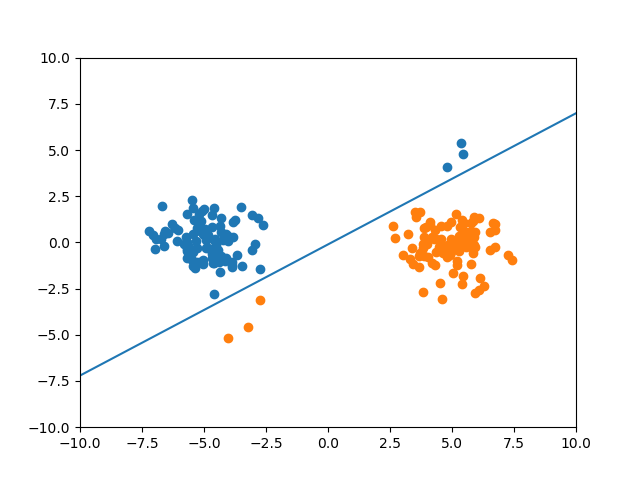
\includegraphics[clip, width=12cm]{../figures/assignment2_result}
    \caption{境界及び点群}
    \label{fig:result}
\end{figure}


\end{document}
